\documentclass[../main]{subfiles}
\begin{document}
% \setcounter{section}{0}
\section{確率}
%------------------------------------------------------------
\begin{minipage}{.5\textwidth}
    \begin{center}
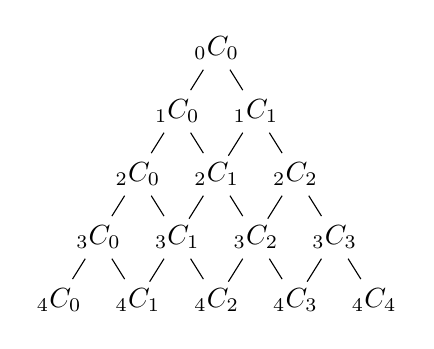
\begin{tikzpicture}[
    level distance=8mm, sibling distance=10mm
    ]
    \node{${}_0C_0$}
    child { node {${}_1C_0$}
        child { node {${}_2C_0$}
            child { node {${}_3C_0$} 
                child { node{${}_4C_0$} }
                child { node{${}_4C_1$} }
            }
            child { node {${}_3C_1$}
                child { node {\phantom{3}} }
                child { node {${}_4C_2$} }
            }
        }
        child { node {${}_2C_1$}
            child { node {\phantom{3}} }
            child { node {${}_3C_2$}
                child { node{\phantom{6}} }
                child { node{${}_4C_3$} }
            }
        }
    }
    child { node {${}_1C_1$}
        child { node {\phantom{2}} }
        child { node {${}_2C_2$}
            child { node {\phantom{3}} }
            child { node {${}_3C_3$} 
                child { node{\phantom{4}} }
                child { node{${}_4C_4$} }
            }
        }
    };
    \end{tikzpicture}
    \hspace{1.6cm} (a)
\end{center}
\end{minipage}
\hfill
\begin{minipage}{.5\textwidth}
    \begin{center}
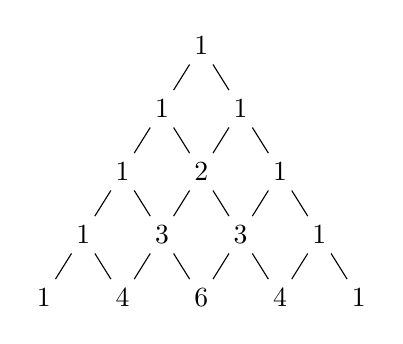
\begin{tikzpicture}[
level distance=8mm, sibling distance=10mm
]
\node{1}
child { node {1}
    child { node {1}
        child { node {1} 
            child { node{1} }
            child { node{4} }
        }
        child { node {3}
            child { node {\phantom{3}} }
            child { node {6} }
        }
    }
    child { node {2}
        child { node {\phantom{3}} }
        child { node {3}
            child { node{\phantom{6}} }
            child { node{4} }
        }
    }
}
child { node {1}
    child { node {\phantom{2}} }
    child { node {1}
        child { node {\phantom{3}} }
        child { node {1} 
            child { node{\phantom{4}} }
            child { node{1} }
        }
    }
};
\end{tikzpicture}
\hspace{1.6cm} (b)
\end{center}
\end{minipage}
%------------------------------------------------------------
\def\firstcircle{(0,0) circle (1.5cm)}
\def\secondcircle{(0:2cm) circle (1.5cm)}
\colorlet{circle edge}{blue!50}
\colorlet{circle area}{blue!20}
\tikzset{filled/.style={fill=circle area, draw=circle edge, thick}, outline/.style={draw=circle edge, thick}}
%------------------------------------------------------------
%\setlength{\parskip}{5mm}
\begin{figure}[H]
    \centering
    \begin{minipage}{.4\textwidth}
        \begin{tikzpicture}[scale=.7]
            \draw[filled] \firstcircle node {$A$};
            \draw \secondcircle node {$B$};
            \draw[outline] \secondcircle;
        \end{tikzpicture}
    \end{minipage}
    \begin{minipage}{.4\textwidth}
        \begin{tikzpicture}[scale=.7]
            \draw \firstcircle node {$A$};
            \draw[filled] \secondcircle node {$B$};
            \draw[outline] \firstcircle;
        \end{tikzpicture}
    \end{minipage}
\end{figure}
%------------------------------------------------------------
% Set A or B
\begin{figure}[H]
    \centering
    \begin{tikzpicture}[scale=.7]
        \draw[filled] \firstcircle node {$A$}
                    \secondcircle node {$B$};
        \node[anchor=south] at (current bounding box.north) {$A\cup B$};
    \end{tikzpicture}
\end{figure}
%------------------------------------------------------------
% Set A or B
\begin{figure}[H]
    \centering
    \begin{tikzpicture}[scale=.7]
        \begin{scope}
            \clip \firstcircle;
            \fill[filled] \secondcircle;
        \end{scope}
        \draw[outline] \firstcircle node {$A$};
        \draw[outline] \secondcircle node {$B$};
        \node[anchor=south] at (current bounding box.north) {$A \cap B$};
    \end{tikzpicture}
\end{figure}
%------------------------------------------------------------
\begin{figure}[H]
    \centering
\begin{tikzpicture}
    \begin{axis}[
        width=8cm, height=5cm,
        samples=200,
        minor x tick num = 0,
        minor y tick num = 0,
        axis x line=bottom,
        axis y line=middle,
        xmin=-1, xmax=8,
        ymin=0, ymax=0.8,
        xlabel=$x$, ylabel=$f(x)$,
        xlabel style={at={(1,0)}, anchor=north west},
        ylabel style={rotate=0, at={(0.15,1)}, anchor=south east},
        xtick={0,1,2,3,4,5},
        ytick={},
        yticklabels={}
    ]
    \addplot[red,thick,domain=0:7,name path=g1] {x*exp(-x)};
    \path[name path=l1] (2,0) -- (2,10);
    \path[name intersections={of=g1 and l1}];
    \addplot[gray,domain=2:7,draw=none,fill=gray!40]{x*exp(-x)} \closedcycle;
    \draw (intersection-1) -- (2,0);
    %\draw (2,0) node[below]{$\mu$};
    \end{axis}
    \draw (2.15,-0.5) node[below]{$\mu$};
\end{tikzpicture}
\caption{指数分布の期待値}
\label{ch_13_1}
\end{figure}
%------------------------------------------------------------
\begin{figure}[H]
    \begin{minipage}[b]{0.49\textwidth}
        \centering
        \begin{tikzpicture}[domain=-4:4,samples=200,scale=0.6]
            \begin{axis}[%
                minor tick num = 0,
                % axis x line = bottom,
                % axis y line = none,
                axis lines=middle,
                % axis line style=thick,
                xmin=-4.0, xmax=4.0,
                ymin=0, ymax=1.0,
                ticks=none,
                % xlabel=$x$,
                every axis x label/.style={at={(current axis.right of origin)},anchor=north west},
                clip=false
            ]
            \addplot [smooth, red, thick, name path=f] {normpdf(x,0,1)};

            \path (0,0) coordinate (MX);
            \path (0,1) coordinate (MY);
            \path (-1.5,0) coordinate (X1);
            \path (-1.5,1) coordinate (Y1);
            \path (1.5,0) coordinate (X2);
            \path (1.5,1) coordinate (Y2);

            \draw (MX) node[below]{$\mu$};

            \path[name path=l] (X1) -- (Y1);
            \path[name intersections={of=f and l}];
            \path (intersection-1) coordinate (A1);
            \draw[dashed] (X1) node[below]{$\mu-\sigma$} -- (A1);

            \path[name path=l] (X2) -- (Y2);
            \path[name intersections={of=f and l}];
            \path (intersection-1) coordinate (A2);
            \draw[dashed] (X2) node[below]{$\mu+\sigma$} -- (A2);

            \draw[<->] (A1) -- node[below left]{$2\sigma$} (A2);

        \end{axis}
        \end{tikzpicture}
        \subcaption{$\sigma$が大きい時}
    \end{minipage}
    \hfill
    \begin{minipage}[b]{0.49\textwidth}
        \centering
        \begin{tikzpicture}[domain=-4:4,samples=200,scale=0.6]
            \begin{axis}[%
                minor tick num = 0,
                % axis x line = bottom,
                % axis y line = none,
                axis lines=middle,
                % axis line style=thick,
                xmin=-4.0, xmax=4.0,
                ymin=0, ymax=1.0,
                ticks=none,
                % xlabel=$x$,
                every axis x label/.style={at={(current axis.right of origin)},anchor=north west},
                clip=false
            ]
            \addplot [smooth, red, thick, name path=f] {normpdf(x,0,0.5)};

            \path (0,0) coordinate (MX);
            \path (0,1) coordinate (MY);
            \path (-0.7,0) coordinate (X1);
            \path (-0.7,1) coordinate (Y1);
            \path (0.7,0) coordinate (X2);
            \path (0.7,1) coordinate (Y2);

            \draw (MX) node[below]{$\mu$};

            \path[name path=l] (X1) -- (Y1);
            \path[name intersections={of=f and l}];
            \path (intersection-1) coordinate (A1);
            \draw[dashed] (X1) node[below]{$\mu-\sigma$} -- (A1);

            \path[name path=l] (X2) -- (Y2);
            \path[name intersections={of=f and l}];
            \path (intersection-1) coordinate (A2);
            \draw[dashed] (X2) node[below]{$\mu+\sigma$} -- (A2);

            \draw[<->] (A1) -- node[below left]{$2\sigma$} (A2);

        \end{axis}
        \end{tikzpicture}
        \subcaption{$\sigma$が小さい時}
    \end{minipage}

    \caption{分散のばらつき}
    \label{ch_13_variance}
\end{figure}
%------------------------------------------------------------
\begin{figure}[H]
    \centering
    \begin{tikzpicture}[domain=0:1,samples=200,scale=0.8]
        \begin{axis}[%
            minor tick num = 0,
            % axis x line = bottom,
            % axis y line = none,
            axis lines=middle,
            % axis line style=thick,
            xmin=0, xmax=1.01,
            ymin=0, ymax=4.0,
            ticks=none,
            % xlabel=$x$,
            every axis x label/.style={at={(current axis.right of origin)},anchor=north west},
            clip=false
        ]
        \addplot [smooth, red, thick, name path=f] {betapdf(x,4,3)};
        \path[name path=axis] (axis cs:0,0) -- (axis cs:1,0);
        % \addplot [domain=0:0.5,smooth, blue, thick,fill=gray!20] {betapdf(x,4,3)} \closedcycle;
        \addplot [fill=gray,fill opacity=0.2] fill between[of=f and axis,soft clip={domain=0.0:0.57-0.2}];
        \addplot [fill=gray,fill opacity=0.2] fill between[of=f and axis,soft clip={domain=0.57+0.2:1}];

        \path (0.57,0) coordinate (MX);
        \path (0.57,3) coordinate (MY);
        \path ($(MX)+(-0.2,0)$) coordinate (X1);
        \path ($(MY)+(-0.2,0)$) coordinate (Y1);
        \path ($(MX)+(0.2,0)$) coordinate (X2);
        \path ($(MY)+(0.2,0)$) coordinate (Y2);

        \draw[dashed] (MX) node[below]{$\mu$} -- (MY);
        \path[name path=l] (X1) -- (Y1);
        \path[name intersections={of=f and l}];
        \path (intersection-1) coordinate (A);
        \draw (X1) node[below]{$\mu-k\sigma$} -- (A);

        \path[name path=l] (X2) -- (Y2);
        \path[name intersections={of=f and l}];
        \path (intersection-1) coordinate (A);
        \draw (X2) node[below]{$\mu+k\sigma$} -- (A);

        \draw[<->] ($(X1)+(0,1)$) -- node[below]{$k\sigma$} ($(MX)+(0,1)$);
        \draw[<->] ($(MX)+(0,1)$) -- node[below]{$k\sigma$} ($(X2)+(0,1)$);

    \end{axis}
    \end{tikzpicture}
    \caption{チェビシェフの不等式}
    \label{ch_12_1}
\end{figure}
%------------------------------------------------------------
\begin{figure}[H]
    \centering
    \begin{tikzpicture}[domain=-4:4,samples=200,scale=0.8]
        \begin{axis}[%
            % enlarge x limits=false,
            minor tick num = 0,
            % axis x line = bottom,
            % axis y line = none,
            % axis lines=middle,
            % axis line style=thick,
            axis lines=none,
            xmin=-4.0, xmax=4.0,
            ymin=0, ymax=0.5,
            ticks=none,
            % xlabel=$x$,
            every axis x label/.style={at={(current axis.right of origin)},anchor=north west},
            clip=false
        ]
        \addplot [smooth, red, thick, name path=f] {normpdf(x,0,1)};

        \path (0,0) coordinate (MX);
        \path (0,0.5) coordinate (MY);
        \path (-1,0) coordinate (X1);
        \path (-1,0.5) coordinate (Y1);
        \path (1,0) coordinate (X2);
        \path (1,0.5) coordinate (Y2);
        \path (-2,0) coordinate (X3);
        \path (-2,0.5) coordinate (Y3);
        \path (2,0) coordinate (X4);
        \path (2,0.5) coordinate (Y4);
        \path (-3,0) coordinate (X5);
        \path (-3,0.5) coordinate (Y5);
        \path (3,0) coordinate (X6);
        \path (3,0.5) coordinate (Y6);

        \draw (-4,0) -- (4,0);
        \draw (0,0) -- (0,0.5);

        \draw (MX) node[below]{\footnotesize$\mu$};

        \path[name path=l] (X1) -- (Y1);
        \path[name intersections={of=f and l}];
        \path (intersection-1) coordinate (A1);
        \draw[dashed] (X1) node[below]{\footnotesize$\mu-\sigma$} -- (A1);

        \path[name path=l] (X2) -- (Y2);
        \path[name intersections={of=f and l}];
        \path (intersection-1) coordinate (A2);
        \draw[dashed] (X2) node[below]{\footnotesize$\mu+\sigma$} -- (A2);

        \path[name path=l] (X3) -- (Y3);
        \path[name intersections={of=f and l}];
        \path (intersection-1) coordinate (A3);
        \draw[dashed] (X3) node[below]{\footnotesize$\mu-2\sigma$} -- (A3);

        \path[name path=l] (X4) -- (Y4);
        \path[name intersections={of=f and l}];
        \path (intersection-1) coordinate (A4);
        \draw[dashed] (X4) node[below]{\footnotesize$\mu+2\sigma$} -- (A4);

        \path[name path=l] (X5) -- (Y5);
        \path[name intersections={of=f and l}];
        \path (intersection-1) coordinate (A5);
        \draw[dashed] (X5) node[below]{\footnotesize$\mu-3\sigma$} -- (A5);

        \path[name path=l] (X6) -- (Y6);
        \path[name intersections={of=f and l}];
        \path (intersection-1) coordinate (A6);
        \draw[dashed] (X6) node[below]{\footnotesize$\mu+3\sigma$} -- (A6);

    \end{axis}
    \end{tikzpicture}
    \caption{正規分布の性質}
    \label{ch_21_stdval}
\end{figure}
%------------------------------------------------------------
\begin{tikzpicture}
    \begin{axis}[
        minor tick num = 0,
        axis x line=bottom,
        axis y line=left,
        xmin=0, xmax=7,
        ymin=0, ymax=0.5,
        ytick=data,
        yticklabel={$\frac{1}{6}$}
    ]
    \addplot+[thick,ycomb,dashed] plot coordinates
        {(1,1/6) (2,1/6) (3,1/6) (4,1/6) (5,1/6) (6,1/6)};
    \end{axis}
\end{tikzpicture}
%------------------------------------------------------------
\begin{tikzpicture}
    \begin{axis}[
        samples=7,
        minor x tick num = 0,
        minor y tick num = 2,
        axis x line=bottom,
        axis y line=middle,
        xmin=-1, xmax=6.9,
        ymin=0, ymax=1.2,
        xtick={0,1,2,3,4,5,6},
        ytick={0,0.5,1},
        yticklabels={,$\frac{1}{2}$,$1$}
    ]
    \addplot+[thick,jump mark left,domain=1:6.91] {x*1/6};
    \end{axis}
    \draw[very thick, blue](-1,0) -- (1.7,0) circle (2pt);
   
\end{tikzpicture}
%------------------------------------------------------------
\begin{center}
    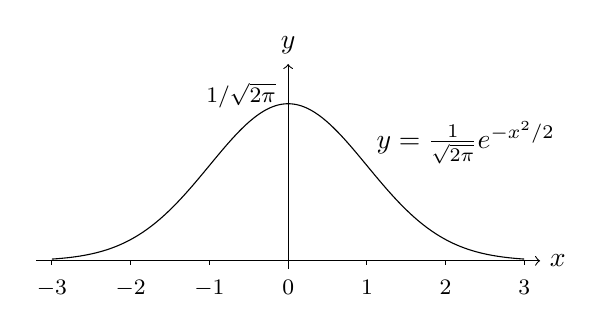
\begin{tikzpicture}[domain=-3:3,samples=200]
    \draw [->] (-3.2,0) -- (3.2,0) node[right] {$x$};
    \draw [->] (0,-0.1) -- (0,2.5) node[above] {$y$};
    \draw plot (\x, {5 * exp(-0.5 * \x * \x) / sqrt(2 * pi)});
    \foreach \x in {-3,...,3}
    \draw (\x,0)--(\x,-0.05) node[below=2pt] {\footnotesize $\x$};
    \draw (0,2.1) node[left=1pt] {\footnotesize $1/\sqrt{2\pi}$};
    2
    \draw (1,1.5) node[above,right] {$y=\frac{1}{\sqrt{2\pi}}e^{-x^2/2}$};
    \end{tikzpicture}
\end{center}
%------------------------------------------------------------
\begin{center}
    \begin{tikzpicture}[domain=-3:3,samples=200]
    \draw [->] (-3.2,0) -- (3.2,0) node[right] {$x$};
    \draw [->] (0,-0.1) -- (0,2.5) node[above] {$y$};
    \draw plot (\x, {1/(sqrt(2*pi*1.5))*exp((-1*\x*\x)/(2*1.5))});
    \foreach \x in {-3,...,3}
    \draw (\x,0)--(\x,-0.05) node[below=2pt] {\footnotesize $\x$};
    \draw (0,2.1) node[left=1pt] {\footnotesize $1/\sqrt{2\pi}$};
    2
    \draw (1,1.5) node[above,right] {$y=\frac{1}{\sqrt{2\pi}}e^{-x^2/2}$};
    \end{tikzpicture}
\end{center}
%------------------------------------------------------------
% https://tex.stackexchange.com/questions/60950/how-to-draw-cdf-of-normal-distribution-in-tikz
\begin{tikzpicture}
    \begin{axis}[%
      xlabel=$x$,
      ylabel=$\CDF(x)$,
      grid=major,
      legend entries={gnuplot, Bowling et al},
      legend pos=south east]
      \addplot [smooth, black] {normcdf(x,0,2)};
    \end{axis}
    \end{tikzpicture}
%------------------------------------------------------------
%------------------------------------------------------------
%------------------------------------------------------------
%------------------------------------------------------------
%------------------------------------------------------------
%------------------------------------------------------------
\end{document}